\chapter{Experimental Evaluation}
\label{chap:experiments}

\section{Evaluation Questions and Recorded Cohorts}
Three evaluations connect the generated skill to its observed execution and processing result. E1 varies the strategy provider and includes an additional rule-feed diagnostic (RQ1). E2 separates learning target force from observing measured force (RQ2). E3 reuses the same C policy at registered positions and directions and measures saved-image ink-area reduction (RQ3). These are distinct cohorts and outcome definitions.

The original E1 cohort is the nominal development session
\begin{quote}\small\path{E1_CT_pass_height_v2_nominal_dev_20261015}\end{quote}
The frozen configuration is \path{e1ct_46de718a23a2a7cf}. It uses evaluator \path{pass_height_ref_v2} and observer \path{received_observations_v2}. Each of its 15 original planned slots has one started execution, five per method, with no retry or exclusion. Five blocks each contain R/T/C in the recorded shuffled order (seed 20261014). C5 is preserved; later C6 is a separate diagnostic. The additional \(R^{*}\) consists of one 19 October diagnostic followed by four extension runs on the same date. It is not part of the original randomized blocks, and R and \(R^{*}\) are never pooled as \(n=10\).

E2 retains all 15 attempts from 13 October, five each in actual order A, B, then C. A4's task outcome follows the operator's field correction: contact release was not completed and the operator interrupted sustained contact. Its software events and stop time are preserved.

E3's image-report selection contains 25 runs, N/P1/P2/D1/D2 with five each. The main thesis evaluation uses N/P1/D1/D2, totaling \EthreeMainN{} selected runs and \EthreeImageN{} image-evaluable pairs. P2 remains five executed archive records, all occluded at the final image. D1-4 remains a selected D1 run but has no whole-stain removal value. These denominators describe inclusion and image support, not a common completion rate.

E1/E2 statistics are calculated from archived per-run precision CSVs matched to the frozen run lists. The additional \(R^{*}\) data include the original run identities and unrounded values. E3 integer areas are reproduced from the original RGB pairs with the saved annotations, ROI, and segmentation algorithm, and compared pixel by pixel with the stored masks. The supplied results manifest links each outcome to its cohort and source; Appendix~\ref{app:e3_archive} documents the reproduction level.

\section{Platform and Metric Boundaries}
The local task uses the UR10 platform, robot-mounted processing tool, and marked plate visible in RGB. The original E1 report identifies UR10 CB3 and an AIDIN AFT200-D80 force/torque sensor. E1/E2 share their respective archived command-processing and lower-level feedback configurations, while E3 retains condition-specific termination and return implementations. Measured spindle RPM, abrasive state, specimen alloy, scratch depth, mass loss, and roughness change are not independently supplied by these records.

E1 time is \texttt{execution\_start} to the first \texttt{TASK\_COMPLETED}, including approach and exit but excluding initial PTP and later HOME. Its \(J_{\mathrm{excess}}\) uses the same whole execution window and the empirical teaching reference \ForceExposureReference~N. E2 completed time is the operator-based interval, with A4 completion null and its interruption interval retained. E3's primary outcome is Equation~\eqref{eq:e3_removal}; neither E1/E2 timing nor E3 automatic diagnostics supply a removal-completion timestamp. Means and sample SD use runs as the sample unit, not frames or pixels.

Table~\ref{tab:expert_il_baselines} summarizes the strategy and force interfaces.

\begin{table}[tbp]\centering\small
\caption[Strategy and information configurations]{Strategy and force interfaces. All retain actual lower-level force feedback. Table~\ref{tab:e2_information_contracts} distinguishes E2 observations from supervision.}
\label{tab:expert_il_baselines}
\begin{tabularx}{\linewidth}{lP{.18\linewidth}X}
\toprule Study & Condition & Strategy and force interface \\ \midrule
E1 & R / \(R^{*}\) & Rule path, +18 N recipe; original / additional processing retiming. \\
 & T & Episode 29 pose/force/source-time replay, scaling 1.0. \\
 & C & Observation-conditioned Flow pose--force chunks. \\
E2 & A & Pose learning; external 23 N target. \\
 & B & Pose--force learning; normalized measured-force inputs masked. \\
 & C & Pose--force learning with measured-force observation/history. \\
E3 & C & Same checkpoint and normalizer; center-relative placement and D-condition direction adapter. \\
\bottomrule
\end{tabularx}
\end{table}

\FloatBarrier
\section{E1: Strategy Comparison}
\label{sec:e1_results}
Figure~\ref{fig:e1_primary_metrics} shows the individual E1 outcomes. Table~\ref{tab:e1_primary} presents the \(R^{*}\)/T/C summary while explicitly retaining their collection dates. Each strategy completes the required procedure in its observed five runs. The original R also completes 5/5 and is preserved alongside \(R^{*}\) in Table~\ref{tab:e1_r_retiming} and the original R/T/C individual outcomes in Appendix~\ref{app:runs}.

\begin{table}[H]\centering\footnotesize\setlength{\tabcolsep}{3pt}
\caption[E1 strategy summary]{E1 strategy summary: \(R^{*}\) is the separate additional five-run diagnostic on 19 October 2026; T/C are the original five each on 15 October. The 15 displayed runs were not randomized together in a new common block. Time and excess integral are mean \(\pm\) sample SD, \(n=5\) per cell. Original R is retained separately; C5 remains included and C6 excluded.}
\label{tab:e1_primary}\begin{tabular}{llcrr}
\toprule
Method & Date / cohort & Done/run & Time (s) & $J_{\mathrm{excess}}$ (N\,s) \\
\midrule
$R^{*}$ & 19 Oct / additional & 5/5 & $24.840 \pm 1.321$ & $0.000 \pm 0.000$ \\
T & 15 Oct / original & 5/5 & $12.897 \pm 0.041$ & $0.125 \pm 0.254$ \\
C & 15 Oct / original & 5/5 & $13.420 \pm 2.630$ & $1.440 \pm 2.785$ \\
\bottomrule
\end{tabular}

\end{table}

\figfull{e1_latest_metrics.pdf}{E1 individual runs and mean \(\pm\) sample SD. Original R, additional \(R^{*}\), original T, and original C are kept separate, with dates on the axis. Each colored point is one run; R*1 and C5 identify the retained short first additional run and high-exposure original C5. C6 is excluded. \(R^{*}\) points and summaries use the verified unrounded per-run CSV; displayed numbers are rounded only for presentation. Bars are dispersion, not confidence intervals.}{fig:e1_primary_metrics}

T has a shorter mean completion time and smaller time SD than C: \EoneTTime\(\pm\)\EoneTTimeSD~s versus \EoneCTime\(\pm\)\EoneCTimeSD~s. Their mean excess integrals are \EoneTExcess{} and \EoneCExcess~N\,s, respectively; \(R^{*}\) and original R have zero observed excess. The common \(Q_{95}\) is a teaching-derived analysis reference, not a target force or safety/damage boundary. These outcomes establish procedure execution and different time--force characteristics. They do not measure ink-removal success or surface quality.

\FloatBarrier
\subsection{Original R and Additional Processing Retiming}
\begin{table}[H]\centering\footnotesize
\caption[Original R and additional R retiming]{Original R and separate additional \(R^{*}\), five runs each. Peak feed is a source-path parameter; measured pass speed is calculated on the successful loaded-pass support. Values are mean \(\pm\) sample SD where appropriate. The dates identify distinct collections.}
\label{tab:e1_r_retiming}\begin{tabular}{lrr}
\toprule
Metric & Original R (15 Oct) & Additional $R^{*}$ (19 Oct) \\
\midrule
Completed / executed & 5/5 & 5/5 \\
Peak-feed parameter (mm/s) & 10.000000 & 14.940779 \\
Completion time (s) & $29.537 \pm 0.075$ & $24.840 \pm 1.321$ \\
Measured pass XY speed (mm/s) & $7.918 \pm 0.124$ & $10.841 \pm 0.088$ \\
$J_{\mathrm{excess}}$ (N\,s) & $0.000 \pm 0.000$ & $0.000 \pm 0.000$ \\
\bottomrule
\end{tabular}

\end{table}

The additional feed reference is 14.940779233290927 mm/s, the summed XY distance divided by summed source time across the stored Z\(\leq175\) mm work-candidate intervals of 42 unique teaching episodes, including four validation episodes. The report records 4299.093664 mm over 287.742265 s. This is a dataset-derived recipe reference, not an independent held-out setting or a verified physical-contact interval.

That value is applied to the existing rest-to-rest quintic path's \emph{peak-feed parameter}. For the quintic scaling \(10u^3-15u^4+6u^5\), the ratio of peak to source movement-average speed is 1.875; the new source processing average is therefore 7.968416 mm/s. The experiment does not match a constant or measured mean TCP speed to 14.941 mm/s. Actual successful-pass XY speed changes from 7.918\(\pm\)0.124 to 10.841\(\pm\)0.088 mm/s. Teaching candidates, full source processing, and successful robot-pass support have different interval definitions.

Only processing is retimed, from 12.243621 to 8.194767 s. The source approach, force ramps, normal-release paths and durations, +18 N target, common controller, and command limits remain as recorded. Later phase start times shift with the shorter processing phase. Source-plan duration is not actual first-completion time because contact synchronization and observed release/rise timing also contribute.

\(R^{*}\)'s mean completion time is \RstarTimeGain~s (\RstarTimePercent\%) shorter than original R. This is a descriptive comparison of separate-date additional diagnostics. The first added run was observed before extending to five, and its shorter release-confirmation interval is retained. R's time depends on path time parameterization and approach/exit as well as processing. The comparison does not attribute shorter learned execution to faster learning computation, or establish an IL advantage after matched measured speed. Original R/T/C tables, receipt traces, and the C5/C6 diagnostic remain in the appendices.

\FloatBarrier
\section{E2: Force-Information Ablation}
E2 separates the two force roles by comparing A/B/C under the shared execution environment. A learns motion and uses an external constant force; B learns motion and force without policy force conditioning; C learns both with measured-force conditioning. The A/B comparison changes both the action dimension and the learned reference schedule. The B/C comparison retains the action and history architecture while changing force-conditioning information. All three are independently trained single-seed checkpoints.

Figure~\ref{fig:e2_primary_metrics} displays all E2 attempts. Table~\ref{tab:e2_times} applies the corrected field outcome. A has four operator-reported completed attempts and one interrupted attempt. B and C have five operator-reported completed attempts each. A4 remains in the all-attempt statistics and has no successful completion time.

\begin{table}[H]\centering\footnotesize
\caption[E2 corrected completion, timing, and peaks]{E2 results with A4 corrected to incomplete release and operator interruption. Completed-time statistics use A \(n=4\), B/C \(n=5\). Mean observed peak is the mean of the five per-run peaks in every condition, including A4, not the whole-signal mean or pooled maximum. Values are mean \(\pm\) sample SD.}
\label{tab:e2_times}
\begin{tabular}{lccrr}
\toprule
Condition & Done/attempt & Time n & Time (s) & Mean peak (N) \\
\midrule
A & 4/5 & 4 & $17.65 \pm 1.20$ & $31.02 \pm 1.46$ \\
B & 5/5 & 5 & $18.81 \pm 0.40$ & $32.42 \pm 0.76$ \\
C & 5/5 & 5 & $15.83 \pm 0.56$ & $31.26 \pm 1.66$ \\
\bottomrule
\end{tabular}

\end{table}

The completed A intervals average \EtwoATime\(\pm\)\EtwoATimeSD~s (\(n=\EtwoATimeN\)), whereas its all-attempt interval averages \EtwoAInterval\(\pm\)\EtwoAIntervalSD~s (\(n=5\)). B and C both complete five attempts. Their completed intervals are \EtwoBTime\(\pm\)\EtwoBTimeSD~s and \EtwoCTime\(\pm\)\EtwoCTimeSD~s, respectively. A4's successful completion time remains null; its stop time is retained in the five-attempt interval, force, and travel statistics.

The B--C mean difference is \BCSeconds~s. With \(\overline t_B\) and \(\overline t_C\) denoting the respective five completed operator-based intervals, the descriptive percentage is
\begin{equation}
 r_t=\frac{\overline t_B-\overline t_C}{\overline t_B}\,100
     =\BCPercent\%.
 \label{eq:bc_time_difference}
\end{equation}
It describes the recorded operator-based timing difference. It does not establish a causal productivity improvement, equal material removal, or a general benefit across every performance measure.

\figfull{e2_primary_metrics.pdf}{All E2 attempts. A4 is shown as a cross at its interruption time. The time summary marks use completed attempts only. Force peaks and XY travel include all five attempts in each condition. Axes retain the full observed ranges.}{fig:e2_primary_metrics}

Table~\ref{tab:e2_force_travel} reports the corresponding all-attempt force and travel statistics.

\begin{table}[tbp]\centering\footnotesize
\caption[E2 all-attempt force and travel]{E2 all-attempt force and motion statistics, \(n=5\) per condition. ``Peak'' is the mean of per-run measured peaks. Whole-window mean force includes approach and exit and is not a contact-only force-quality measure.}
\label{tab:e2_force_travel}
\begin{tabular}{lrrr}
\toprule
Condition & Mean $F_z^B$ (N) & Peak $F_z^B$ (N) & XY travel (mm) \\
\midrule
A & $12.09 \pm 4.14$ & $31.02 \pm 1.46$ & $229.68 \pm 59.50$ \\
B & $11.40 \pm 1.17$ & $32.42 \pm 0.76$ & $205.84 \pm 4.80$ \\
C & $9.36 \pm 0.48$ & $31.26 \pm 1.66$ & $189.22 \pm 8.60$ \\
\bottomrule
\end{tabular}

\end{table}

The mean measured peaks are similar in scale across A, B, and C; C is not below A in the group mean. Whole-window mean force and XY travel are lower for C in this cohort. The shorter contact interval and different approach/exit timing can explain part of those differences, so lower mean force is not interpreted as more accurate force regulation or more effective material processing.

The mean time with recorded \(F_z^B\geq3\) N is \EtwoAContactTime\(\pm\)\EtwoAContactTimeSD~s for A, \EtwoBContactTime\(\pm\)\EtwoBContactTimeSD~s for B, and \EtwoCContactTime\(\pm\)\EtwoCContactTimeSD~s for C. These existing contact diagnostics describe temporal organization on the observed window; they do not define a new threshold for effective polishing.

Full force traces and transition cases are retained in Appendix~\ref{app:e2_cases}, Figures~\ref{fig:e2_force_all} and~\ref{fig:e2_transition_cases}.


\FloatBarrier
\section{E3: Spatial Transfer of the Learned Skill}
\label{sec:e3_results}
E3 evaluates reuse of the same C checkpoint and normalizer without new teaching or retraining. N is nominal, P1 translates the registered region, and D1/D2 change its in-plane direction while also retaining their small center offsets. Figure~\ref{fig:e3_registered_layout} plots the registered positions and directions. Table~\ref{tab:e3_placements} gives the actual registered values verified in the saved per-run registration and execution contexts. They are registration values rather than independent precision surface measurements.

\begin{table}[H]\centering\small
\caption[E3 actual registered placements]{Main E3 conditions: registered offsets from nominal and direction change. D1/D2 include the listed center shifts. Each value is consistent across the five selected run contexts for its condition.}
\label{tab:e3_placements}\begin{tabular}{lrrr}
\toprule
Condition & $\Delta X$ (mm) & $\Delta Y$ (mm) & $\varphi$ (deg) \\
\midrule
N & 0.00 & 0.00 & 0.00 \\
P1 & +29.55 & +21.80 & 0.00 \\
D1 & -1.06 & -1.36 & +42.17 \\
D2 & -0.75 & -3.53 & -31.03 \\
\bottomrule
\end{tabular}

\end{table}

\figfull{e3_registered_layout.pdf}{Registered center offsets and directions for N/P1/D1/D2. Left axes show the recorded registration offsets in millimeters. Right arrows show direction relative to nominal, with arbitrary display length; they are not measured stroke lengths or tool footprints. Small center shifts in D1/D2 are retained in the table.}{fig:e3_registered_layout}

Position transfer uses center-relative XY and restoration to the live center. D1/D2 additionally align observation XY and the policy image to the teaching reference, then inversely transform generated XY. Z, tool posture, force actions, and measured-force channels are not jointly rotated as a full \(SE(3)\) transform. The result evaluates the policy together with its registration/direction adapter; it does not isolate spontaneous rotation generalization of the policy.

\subsection{Selection and Image Evaluation}
The image report preserves the original 25-run final selection rather than selecting new successful or latest runs. N is from 21 October and the selected P/D executions are from 23 October. P1 combines earlier repeats 2/4 with repeats 1/3/5; P2 includes retries of 1/2/3 and retained 4/5; D1/D2 include the final confirmed repeat-5 retries. The frozen selection manifests and original run identifiers define membership. D1-4 retains its original \texttt{manual\_abort}. The experiment is a selected development collection, not a randomized controlled transfer study.

Table~\ref{tab:e3_main_results} reports the image-area results, and Figure~\ref{fig:e3_removal_metrics} shows every evaluable run. The main removal comparison excludes P2 because every final P2 image is tool-occluded. P2 was executed and remains in the archive. In D1, all five selected runs remain, but D1-4's final tool occlusion prevents whole-stain measurement. Thus the main evaluation contains \EthreeMainN{} selected runs and \EthreeImageN{} evaluable image pairs. The semiautomatic gray-threshold and saved-boundary analysis is defined in Section~\ref{sec:e3_image_method}. The established analysis is reproduced without changing its annotations or pixel criteria.

\begin{table}[H]\centering\footnotesize
\caption[E3 image-based stain-area removal]{Main E3 removal results, mean \(\pm\) sample SD over image-evaluable runs. All conditions contain five selected executions. D1 image \(n=4\) means four evaluable pairs, not a 4/5 success rate; D1-4 is final-tool-occluded. P2's five occluded runs are archived outside this main table.}
\label{tab:e3_main_results}\begin{tabular}{lccrc}
\toprule
Condition & Selected n & Image n & Removal (\%) & Unavailable \\
\midrule
N & 5 & 5 & $100.00 \pm 0.00$ & 0 \\
P1 & 5 & 5 & $97.55 \pm 2.49$ & 0 \\
D1 & 5 & 4 & $98.12 \pm 3.75$ & 1 \\
D2 & 5 & 5 & $93.67 \pm 6.60$ & 0 \\
\bottomrule
\end{tabular}

\end{table}

\figfull{e3_removal_metrics.pdf}{All \EthreeImageN{} evaluable main-run removal percentages with run numbers, condition means, and sample SD. D1-4 has no point and no imputed percentage. The full observed range includes D2-3 at 83.879\%. Mean/SD are calculated over runs, without pooling pixels or defining a removal-success threshold.}{fig:e3_removal_metrics}

Condition means range from \EthreeDtwoRemoval\% (D2) to \EthreeNRemoval\% (N). This is a range of \emph{condition means}, not a lower bound for individual runs. D2 includes the 83.879\% observation, and D1-4 and P2 remain unquantified. A 100\% value denotes no residual black ink detected at the original image resolution and established segmentation criterion.

Figures~\ref{fig:e3_first_index_evidence} and~\ref{fig:e3_direction_evidence} show first-index original RGB and unchanged masks at identical scale. Appendix~\ref{app:e3_archive} retains the occluded D1-4/P2 records and lowest observed removal, D2-3.

\begin{figure}[p]\centering
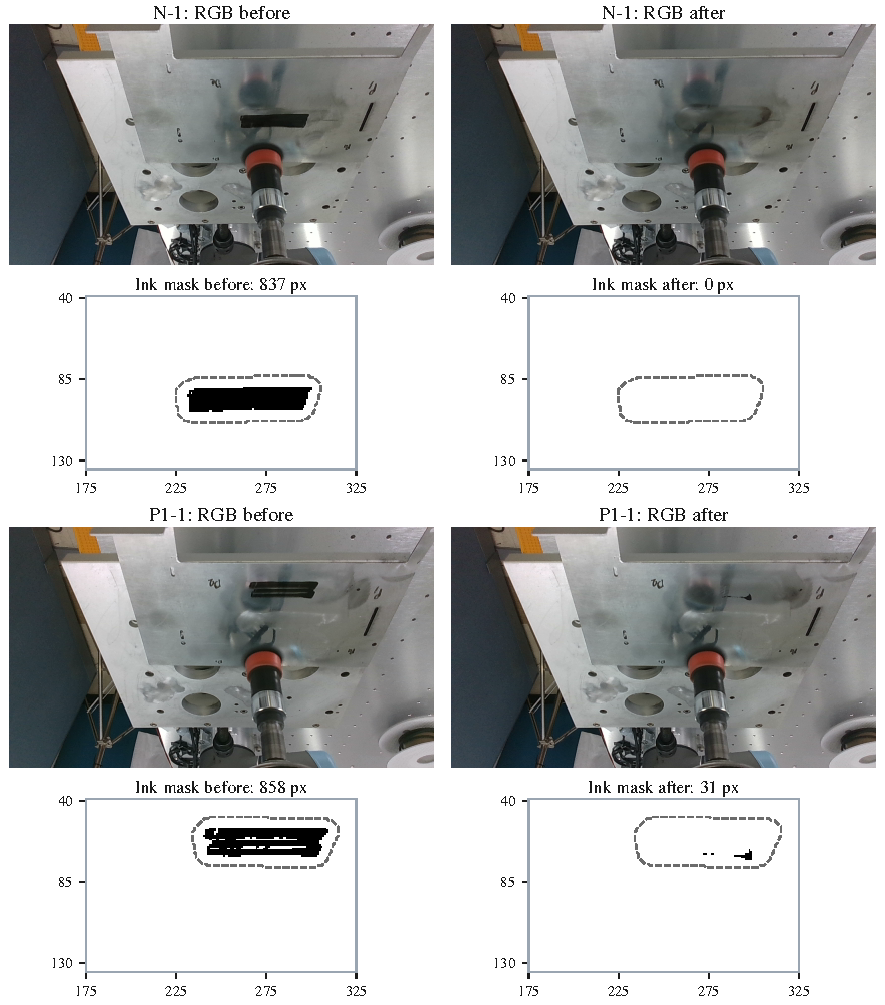
\includegraphics[width=\linewidth]{figures/e3_first_index_evidence_np.pdf}
\caption[E3 N/P1 original RGB and ink masks]{N-1 and P1-1: original before/after RGB and enlarged binary ink masks. Black denotes counted ink; the dashed outline is the unchanged ROI. Mask axes are native pixel coordinates and use the same crop and scale in every example. No residual is detected in N-1; P1-1 retains 31 pixels. Original RGB resolution is \(424\times240\); enlargement adds no image detail.}
\label{fig:e3_first_index_evidence}
\end{figure}

\begin{figure}[p]\centering
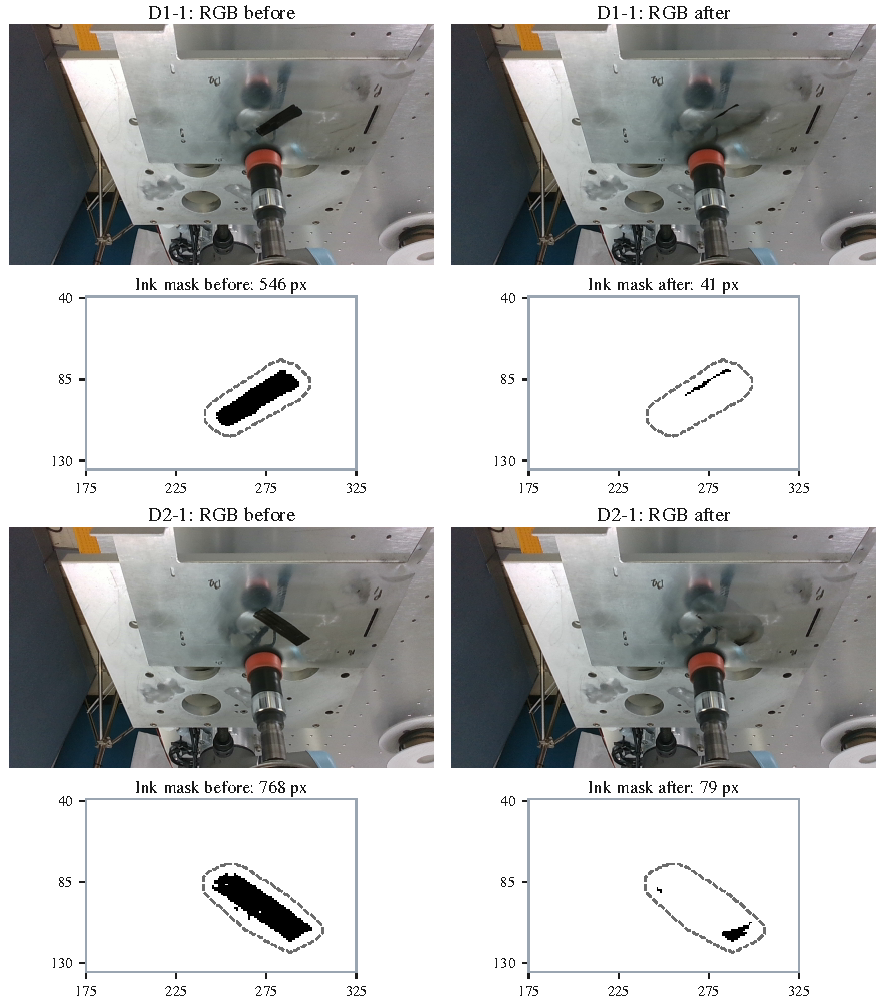
\includegraphics[width=\linewidth]{figures/e3_first_index_evidence_d.pdf}
\caption[E3 D1/D2 original RGB and ink masks]{D1-1 and D2-1: original before/after RGB and saved binary masks, displayed with the same rules as Figure~\ref{fig:e3_first_index_evidence}. The original remaining ink pixels are retained. Measured areas come from native images and masks, independently of the display enlargement.}
\label{fig:e3_direction_evidence}
\end{figure}

\FloatBarrier
\section{Answers to the Research Questions}
For RQ1, the original R/T/C and separate additional \(R^{*}\) each complete the defined procedure in their observed five runs. T has a shorter mean completion time and smaller time SD than C, while C has greater excess-force integral. \(R^{*}\) illustrates sensitivity to rule-path time parameterization without replacing the original experiment or establishing a matched-speed learning advantage.

For RQ2, B/C both complete five attempts and C has a \BCSeconds~s (\BCPercent\%) shorter mean operator-based completion interval. A completes four of five, retaining A4 as an interrupted release transition. The separately trained single-seed configurations change target-force learning and/or force conditioning; they do not establish a general causal effect or a monotonic advantage across all metrics.

For RQ3, the same policy and task-registration/direction adapter yield observed condition-mean image-area removal of \EthreeDtwoRemoval--\EthreeNRemoval\% across the evaluable N/P1/D1/D2 images. This supports reuse within the tested placements. It does not establish arbitrary-shape, curved-surface, or height robustness, superiority over R/T, or a causal spatial-transfer effect of force observation. E3 adds ink-area evidence without retrospectively measuring E1/E2 removal quality.
